\documentclass{article}
\usepackage{graphicx}
\graphicspath{ {images/} }

\title{Dynamic sampling pointnet notes}
\author{xyz}
\date{Feb 2018}

\begin{document}
%\tableofcontents{}
\begin{titlepage}
\maketitle
\end{titlepage}	

\section{Quick notes for important events while using one file to test}
\subsection{batch size}
\subsubsection{bs=27 vs bs=81}
batch size: 9,27,81 \par
data: xyz-color\_1norm\par
model: 1AG\par
sampling \& grouping: stride\_0d1\_step\_0d1\_bmap\_nh5\_2048\_0d5\_1\_fmn1-160\_32-32\_12-0d2\_0d6-0d2\_0d6\par
\begin{figure}[h]
	\caption{bs=9}
	\centering
	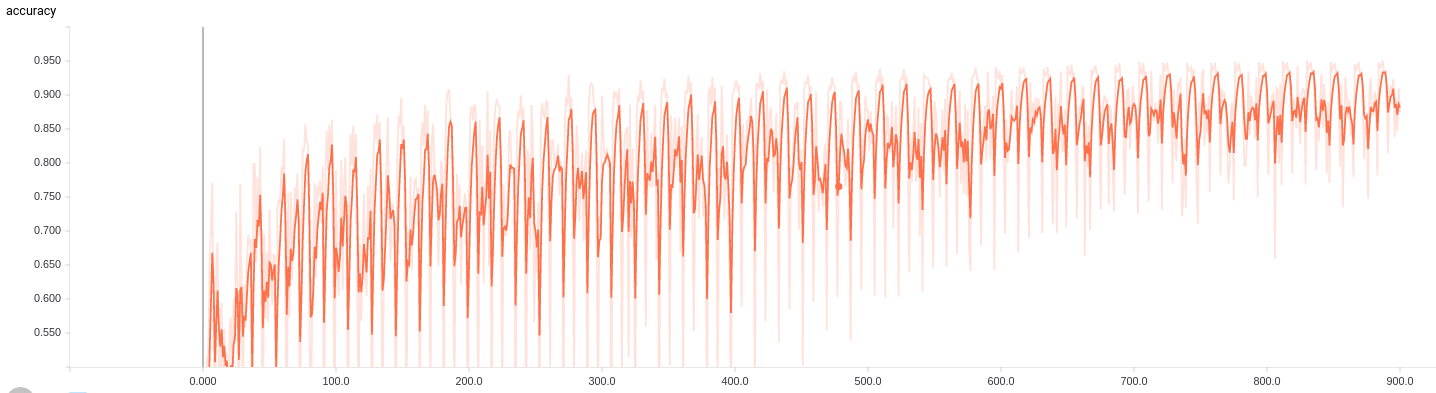
\includegraphics[width=\textwidth]{acc_log-model_1AG-gsbb_2C1-bs9-xyz-color_1norm-2048-mat}
	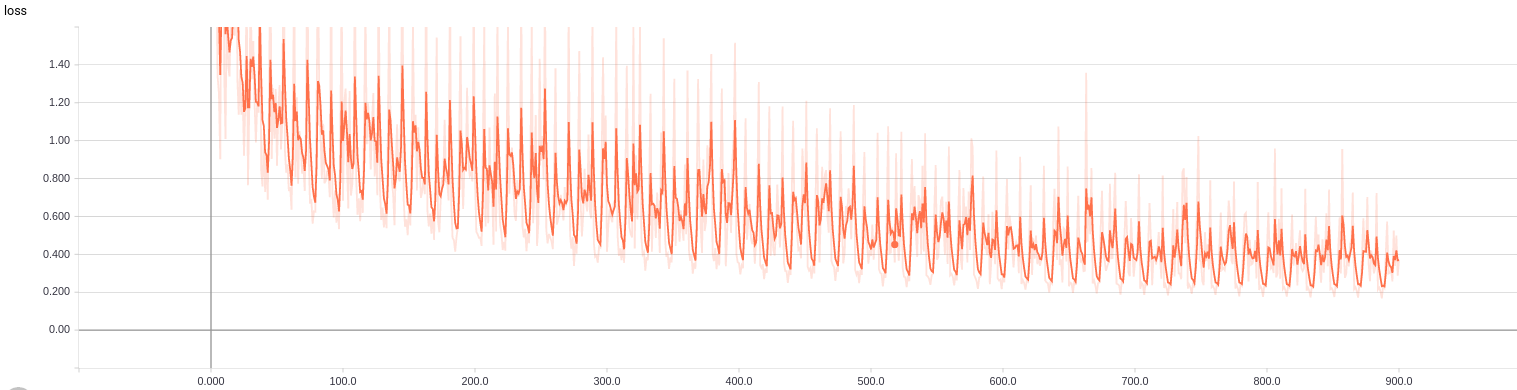
\includegraphics[width=\textwidth]{loss_log-model_1AG-gsbb_2C1-bs9-xyz-color_1norm-2048-mat}
\end{figure}
\begin{figure}[h]
	\caption{bs=27}
	\centering
	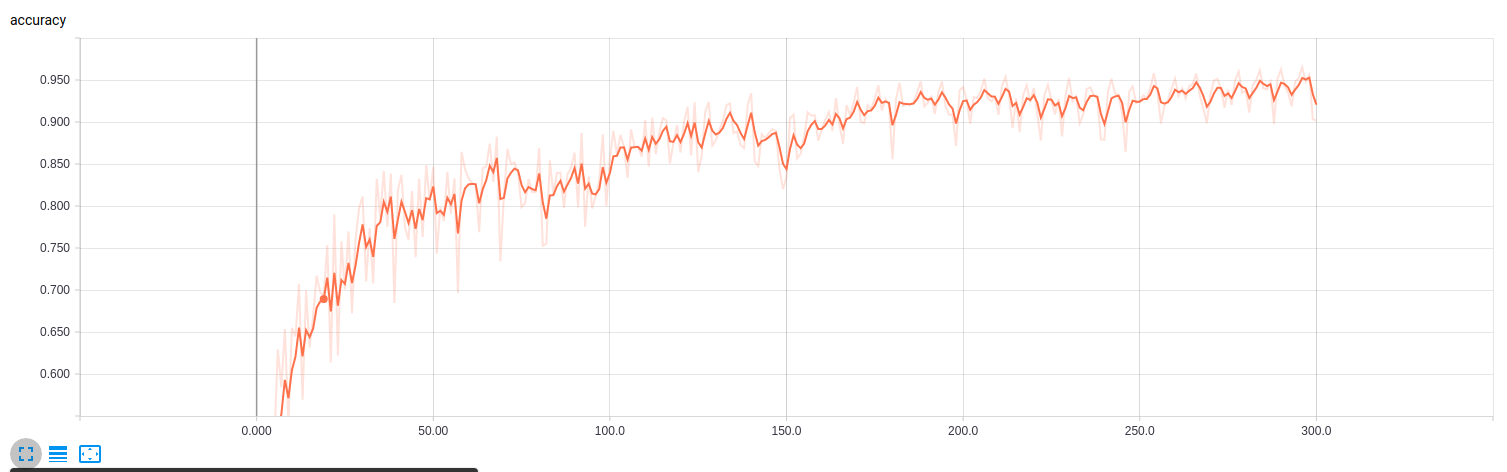
\includegraphics[width=\textwidth]{acc_log-model_1AG-gsbb_2C1-bs27-xyz-color_1norm-2048-mat}
	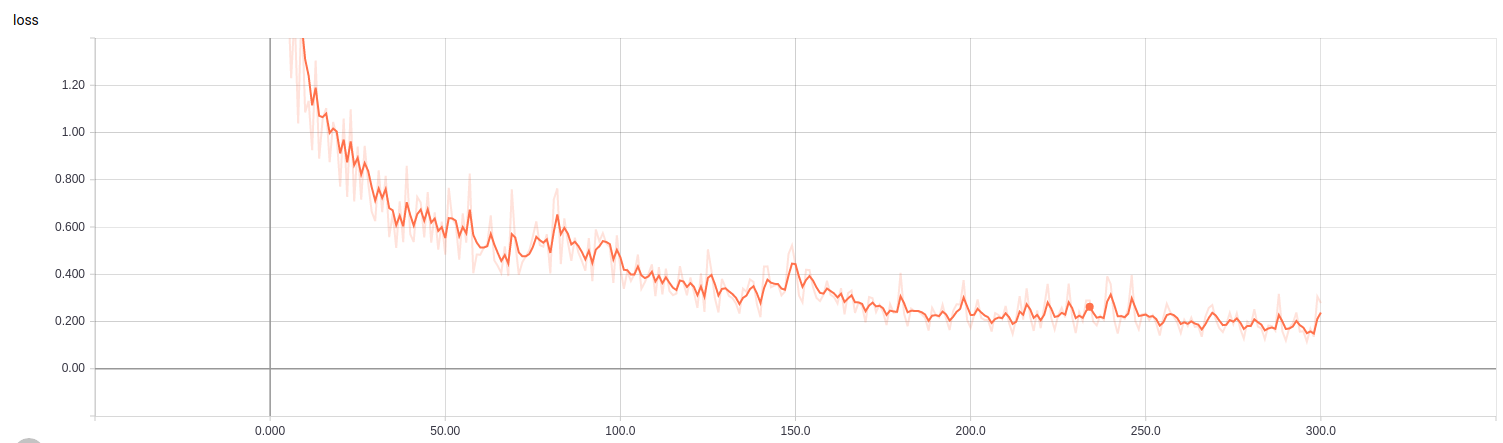
\includegraphics[width=\textwidth]{loss_log-model_1AG-gsbb_2C1-bs27-xyz-color_1norm-2048-mat}
\end{figure}
\begin{figure}[h]
	\centering
	\caption{bs=81}
	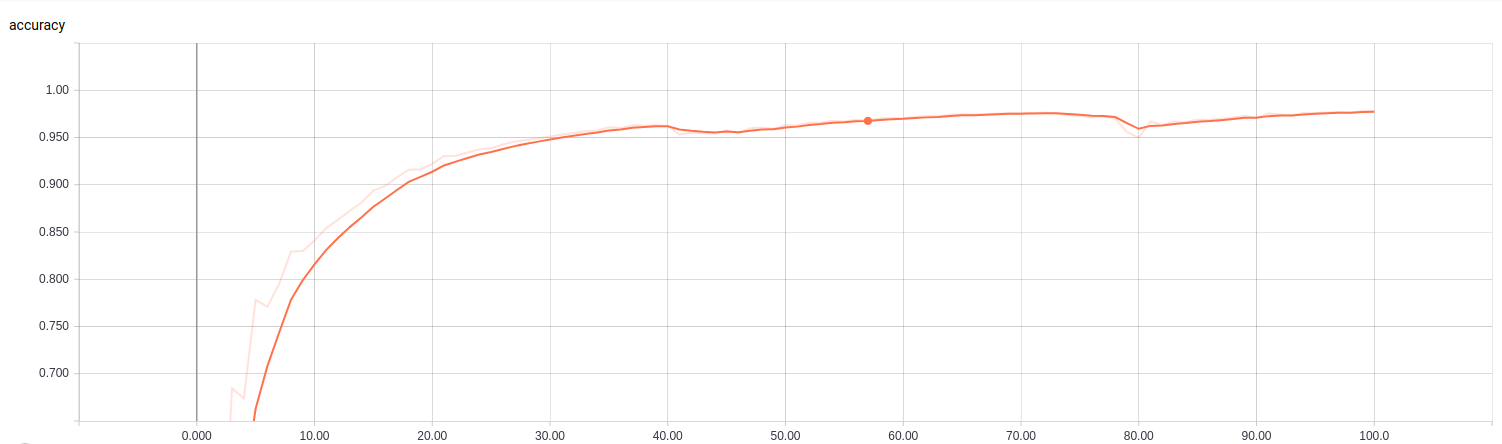
\includegraphics[width=\textwidth]{acc_log-model_1AG-gsbb_2C1-bs81-xyz-color_1norm-2048-mat}
	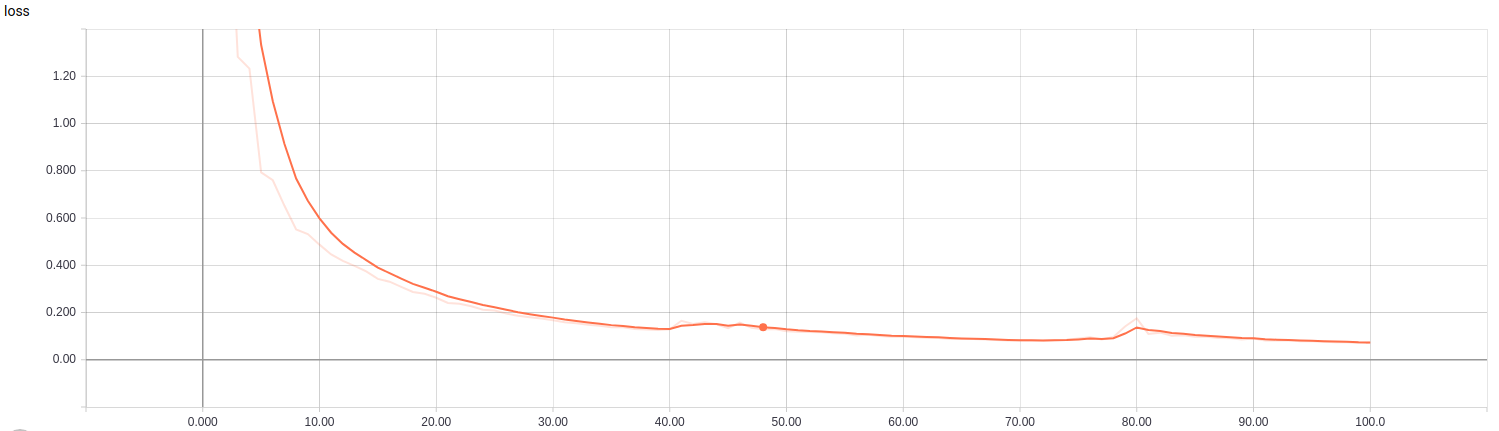
\includegraphics[width=\textwidth]{loss_log-model_1AG-gsbb_2C1-bs81-xyz-color_1norm-2048-mat}
\end{figure}
\subsection{feed elements}
epoch num = 100
\begin{center}
	\begin{tabular}{|c | c || c c |} 
		\hline
		batch size & data elements & acc & loss \\
		\hline
		9 & xyz color & 0.890 & 0.356\\ [0.5ex] 
		\hline
		27 & xyz color & 0.920 & 0.240\\ [0.5ex] 
		\hline
		81 & xyz color & 0.978 & 0.072\\ [0.5ex] 
		\hline
		9 & xyz  & 0.861 & 0.427\\ [0.5ex] 
		\hline
		27 & xyz & 0.907 & 0.257\\ [0.5ex] 
		\hline
		81 & xyz & 0.975 & 0.078 \\  [1ex] 
		\hline
	\end{tabular}
\end{center}
\end{document}